% PACKAGES INCLUDED HERE 
% DO NOT NEED TO CHANGE
\documentclass[conference]{IEEEtran}
%\IEEEoverridecommandlockouts
% The preceding line is only needed to identify funding in the first footnote. If that is unneeded, please comment it out.
\usepackage{cite}
\usepackage{amsmath,amssymb,amsfonts}
\usepackage{algorithmic}
\usepackage{graphicx}
\usepackage{textcomp}
\def\BibTeX{{\rm B\kern-.05em{\sc i\kern-.025em b}\kern-.08em
    T\kern-.1667em\lower.7ex\hbox{E}\kern-.125emX}}
\begin{document}

% TITLE GOES HERE

\title{Parking Lot Manager\\}


\author{\IEEEauthorblockN{Girgis Shihataa}
\IEEEauthorblockA{\textit{Department of Computer Science} \\
\textit{Middle Tennessee State University}\\
Murfreesboro, United States of America \\
grs2w@mtmail.mtsu.edu}
\and
\IEEEauthorblockN{William Smith}
\IEEEauthorblockA{\textit{Department of Computer Science} \\
\textit{Middle Tennessee State University}\\
Murfreesboro United States of America \\
wbs3d@mtmail.mtsu.edu}
\and
\IEEEauthorblockN{Michael Ketzner}
\IEEEauthorblockA{\textit{Department of Computer Science} \\
\textit{Middle Tennessee State University}\\
Murfreesboro, United States of America \\
mdk4g@mtmail.mtsu.edu}
\and
\IEEEauthorblockN{Justin Hill}
\IEEEauthorblockA{\textit{Department of Computer Science} \\
\textit{Middle Tennessee State University}\\
Murfreesboro, United States of America \\
jph5s@mtmail.mtsu.edu}
\and
\IEEEauthorblockN{Mubarek Mohammed}
\IEEEauthorblockA{\textit{Department of Computer Science} \\
\textit{Middle Tennessee State University}\\
Murfreesboro, United States of America \\
mmm9b@mtmail.mtsu.edu}
\and
\IEEEauthorblockN{Carolous Ghobrial}
\IEEEauthorblockA{\textit{Department of Computer Science} \\
\textit{Middle Tennessee State University}\\
Murfreesboro, United States of America \\
cag6p@mtmail.mtsu.edu}
}

\maketitle

% ABSTRACT 

\begin{abstract}
This document is a model and instructions for \LaTeX.
This and the IEEEtran.cls file define the components of your paper [title, text, heads, etc.]. *CRITICAL: Do Not Use Symbols, Special Characters, Footnotes, 
or Math in Paper Title or Abstract.
\end{abstract}


% KEYWORDS

\begin{IEEEkeywords}
component, formatting, style, styling, insert
\end{IEEEkeywords}

% INTRODUCTION SECTION
\section{Introduction and Background}

\subsection{Introduction}
If you are a student at MTSU, Middle Tennessee State University, and you commute, you know the struggles of finding a parking space near your class during the day. MTSU currently has a problem with parking lots for all the students who commute to campus. The number of students commuting to MTSU continues to increase every year and the problem has only increased. This always results in a large number of students funneling into and circling around parking lots at very desired locations on a daily basis. The parking lots can be completely full, but students will continue to drive around hoping they come across an empty spot. Our goal for this project was to build and train a neural network that can help provide a solution for this problem. 

Throughout the length of this project, we went through multiple ideas, or iterations, of the neural network. At first, we quickly recognized that for this project, we need to build and train a CNN, convolutional neural network. The main advantage for building a CNN is that it automatically detects important features without any supervision, thus allowing for more complex networks.\cite{b1} There are many versions of convolutional networks that we researched, but eventually, we ended up with three main prospects: a basic CNN, a Faster R-CNN,or a YOLO-V3. 

Through the basic CNN and the Faster R-CNN, we can achieve our neural network goal by having the neural network look at one vehicle at a time. This means that the network is binary and has the ability to observer if a vehicle is in the picture or not \cite{b1}. This opens up an avenue of methods that we can achieve our goal by. Mainly, the neural network can observe vehicles going and going out of the parking lot, or it can observe the parking lot spaces separately. The former being more efficient in hardware required, and the latter being more accurate.

For the final prospect, the YOLO-V3, our neural network has the ability to detect multiple vehicles in a singular picture \cite{b1}. This network allows us to have the most efficient setup for hardware, a singular camera on top of a post in any of the parking lots. The camera will take an aerial view picture of the entire lot, and the neural network will process the image by going observing how many vehicles are in the parking lot. For obvious reasons, this has the least amount of accuracy, and thus will result in far more errors for our ideal goal.

% BACKGROUND SECTION
\subsection{Background}

Parking at MTSU for students has been a rising issue in the recent years and it seems as if there will not be any solutions offered by the school in the near future. This neural network was built and trained in light of this problem to provide a possible solution. Our plan for this project was to build a neural network that can detect vehicles in a parking lot. For the near future, we hoped that we could get in contact with MTSU's mobile development team in hopes of building an application that will receive input from the neural network as to which parking lots are open and which are full. As of now and the current quarantine situation, this is not possible.

This project can help better the lives of students commuting at MTSU, and potentially even other universities, by lessening the time it takes to find a parking spot. From personal experience amongst our group, we had an average of 15 minutes to find a parking spot, and almost 90 percent of the time, it was no where near our destination building. By reducing the time it takes to find a parking spot and potentially even, at a closer lot to the destination building, this will free any and all future students from the stresses of searching for a parking space and improve the time it takes for them to commute. By reducing commute time, less students will be late because of the traffic in parking lots.

After many deliberations, we finally decided on going through with a basic CNN for three important reasons. 
\begin{itemize}
    \item Simpler implementation 
    \item Less training time/epochs compared to other networks
    \item Accuracy is within acceptable range
\end{itemize}
As listed above, the basic CNN does everything the other networks do as good, if not better. It is also much easier to implement than the other aforementioned networks. 

% METHODS SECTION
\section{Methods}

\subsection{Data}
We decided on using a prepared data-set available online that contains a total of 12584 images.The images have already been formatted in .JPG image format. The images were collected at varying weather conditions as well as different situations of light conditions. The difference in perspective and angles of view creates the capability to train the network with a variety of images. The addition of noise to the images helps improve/prepare the network for future testing.

\subsection{Input Processing}
We downsized the images to an input shape of 150X150 before feeding the images to the network. The image set has been divided into two batches, training and testing image data set. The training data set consists 11326 images. The testing data set consists 1258 images. We normalized the image from a scale of 0.0 to 255.0 to 0.0 to 1.0 float32 value. The normalization makes of the image data reduces the memory utilized. We utilized Keras image preprocessing tools to perform slight transformations on the image that helps in the creation of a stronger and more robust model. We performed preprocessing techniques including rotation range that performs
random rotation of the images, re-scaling factor to reduce the RGB value to range between 0.0 to 1.0, shear range alteration that cuts away part of the image that is deemed non-essential, stretching and fill mode that performs the reshaping of the image which entails the filling of the missing pixels with the nearest value of neighboring pixels (Fig 1). 
\begin{figure}[htbp]
\centerline{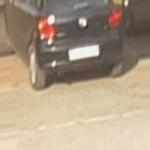
\includegraphics[width=\linewidth]{./random_car_transform.jpg}}
\caption{Pre-processed image of a car.}
\label{fig}
\end{figure}

\subsection{Convolution Neural Networks}
For our neural network architecture, we built a Convolution Neural Network which have been known for providing a higher accuracy of recognition compared to other Neural Network architectures including YOLOv3. We built our network based on further research on well known CNN architectures including LeNet-5 which is designed for large-scale visual recognition problems. In comparison, our architectures is built to fit a smaller scale visual recognition where the solution is binary choice between parking space being empty or full. 

Our architecture accepts an input image shape of 150X150 with a number of channels equal to 3. Our architecture consists of three convolution layers that are essential to extract the visual features of the image. The filters selected for the first and second convolution layers is equal to 32. We increased the filters in the third convolution layer to 64 in order to grab the image features and patterns like corners and edges. We decided upon a kernel size of 3X3 in our layers which
aligns with the objective of capturing the images features.The convolution layers are followed by rectified linear unit activation function (ReLU) and max pooling layers with a pool size of 2X2. We flattened the 3D feature maps to 1D feature vectors. We pass the flatten layer to a dense layer consisting of 64 neurons followed by rectified linear unit activation function (ReLU). We chose a larger number of neuron size to improve the CNN architectures robustness and the ability to extract patterns. The dense layer is followed by another rectified linear unit activation function (ReLU). With the target of reducing over-fitting of the training data-set, we introduced the dropout layer that turns off 50 percent of the neurons randomly during training process. The final dense layer consists of a single neuron which is the representation of the solution of our network. A single neuron represents the fact of the outcome of the network as a 0 or 1 where 0 signals an image of a busy parking space while 1 represents an image of a free parking space. The model is compiled with binary crossentropy loss function which lines with the binary classification problem of our architecture. 
Figure 2 displays the detailed structure of our CNN.

\begin{figure}[htbp]
\centerline{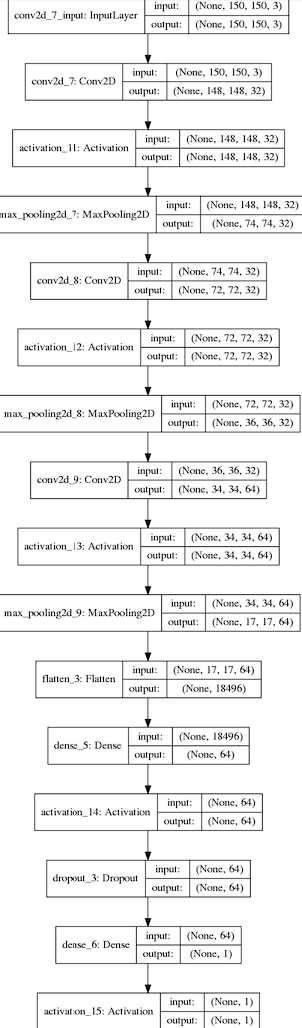
\includegraphics[scale=1]{./model_plt.png}}
\caption{Detailed structure of the CNN.}
\label{fig}
\end{figure}

% RESULTS SECTION
\section{Results}

Start typing here \cite{b4}.

% DISCUSSION SECTION
\section{Discussion}

Start typing here \cite{b5}.

% REFERENCES
% THIS IS CREATED AUTOMATICALLY
\bibliographystyle{IEEEtran}
\bibliography{References} % change if another name is used for References file

\end{document}
